\documentclass[12pt,letterpaper]{article}
\usepackage{graphicx,textcomp}
\usepackage{natbib}
\usepackage{setspace}
\usepackage{fullpage}
\usepackage{color}
\usepackage[reqno]{amsmath}
\usepackage{amsthm}
\usepackage{fancyvrb}
\usepackage{amssymb,enumerate}
\usepackage[all]{xy}
\usepackage{endnotes}
\usepackage{lscape}
\newtheorem{com}{Comment}
\usepackage{float}
\usepackage{hyperref}
\usepackage{pdfpages}
\newtheorem{lem} {Lemma}
\newtheorem{prop}{Proposition}
\newtheorem{thm}{Theorem}
\newtheorem{defn}{Definition}
\newtheorem{cor}{Corollary}
\newtheorem{obs}{Observation}
\usepackage[compact]{titlesec}
\usepackage{dcolumn}
\usepackage{tikz}
\usetikzlibrary{arrows}
\usepackage{multirow}
\usepackage{xcolor}
\newcolumntype{.}{D{.}{.}{-1}}
\newcolumntype{d}[1]{D{.}{.}{#1}}
\definecolor{light-gray}{gray}{0.65}
\usepackage{url}
\usepackage{listings}
\usepackage{color}

\definecolor{codegreen}{rgb}{0,0.6,0}
\definecolor{codegray}{rgb}{0.5,0.5,0.5}
\definecolor{codepurple}{rgb}{0.58,0,0.82}
\definecolor{backcolour}{rgb}{0.95,0.95,0.92}

\lstdefinestyle{mystyle}{
	backgroundcolor=\color{backcolour},   
	commentstyle=\color{codegreen},
	keywordstyle=\color{magenta},
	numberstyle=\tiny\color{codegray},
	stringstyle=\color{codepurple},
	basicstyle=\footnotesize,
	breakatwhitespace=false,         
	breaklines=true,                 
	captionpos=b,                    
	keepspaces=true,                 
	numbers=left,                    
	numbersep=5pt,                  
	showspaces=false,                
	showstringspaces=false,
	showtabs=false,                  
	tabsize=2
}
\lstset{style=mystyle}
\newcommand{\Sref}[1]{Section~\ref{#1}}
\newtheorem{hyp}{Hypothesis}

\title{Problem Set 1}
\date{Due: January 29, 2020}
\author{Farris Sabir QTM 200: Applied Regression Analysis}

\begin{document}
	\maketitle
	
	\section*{Instructions}
	\begin{itemize}
		\item Please show your work! You may lose points by simply writing in the answer. If the problem requires you to execute commands in \texttt{R}, please include the code you used to get your answers. Please also include the \texttt{.R} file that contains your code. If you are not sure if work needs to be shown for a particular problem, please ask.
		\item Your homework should be submitted electronically on the course GitHub page in \texttt{.pdf} form.
		\item This problem set is due at the beginning of class on Wednesday, January 29, 2020. No late assignments will be accepted.
		\item Total available points for this homework is 100.
	\end{itemize}
	
	\vspace{1cm}
	\section*{Question 1 (25 points)}

A private school counselor was curious about the average of IQ of the students in her school and took a random sample of 25 students' IQ scores. The following is the data set:
\vspace{.5cm}

\lstinputlisting[language=R, firstline=41, lastline=41]{PS1.R}  

\vspace{.5cm}

\noindent Find a 90\% confidence interval for the student IQ in the school assuming the population of IQ from which our random sample has been selected is normally distributed. 

\vspace{.5cm}

\lstinputlisting[language=R, firstline=43, lastline=56]{PS1.R}  

\vspace{.5cm}

\noindent The z-scores of 1.71 and -1.71 on both sides of the t distribution corresponded to a 90\% confidence interval. The standard error or standard deviation of the sampling distribution was determined by the sample's standard deviation (denoted by sdIQ) divided by the square root of the sample size. Hence, the product of the z-score and the standard error yielded the margin of error, which is 4.48. The margin of error was added to and subtracted from the mean, which was denoted by meanIQ, to obtain the confidence interval. This interval was verified by the R function t.test.
\noindent Thus, the 90\% confidence interval for the student IQ in the school is 94 to 103. If this was among 100 samples of students' IQ scores, confidence intervals calculated from 95 of them would have the true mean IQ score within them.

\vspace{1cm}
\section*{Question 2 (25 points)}
A private school counselor was curious whether  the average of IQ of the students in her school is higher than the average IQ score 100 among all the schools in the country. She took a random sample of 25 students' IQ scores. The following is the data set:
\vspace{.5cm}
\lstinputlisting[language=R, firstline=67, lastline=67]{PS1.R}  
\vspace{.5cm}

\noindent Conduct a test with 0.05 significance level assuming the population of IQ from which our random sample has been selected is normally distributed:

\vspace{.5cm}

\noindent The conditions meet the assumptions for a t-test because the data was collected from the students using a random sample. Also, the IQ scores of the population are assumed to lie along a normal distribution, as previously stated.

\vspace{.5cm}

\noindent The null hypothesis for this test is that the average IQ score of the students of this private counselor's school is equal to the IQ score of 100, the average for all schools in the country. The alternative hypothesis is that the average IQ score of the students of this counselor's school is greater than the IQ score of 100, the average for all schools in the country.

\vspace{.5cm}

\noindent Because the population of IQ scores is normally distributed, the sampling distribution of sample mean ybar is normal about mu or the population mean or average IQ score of students in the school of the counselor. To assess how far this population mean deviates from the national mean IQ score of 100, the standard error denoted as SE must be calculated. Therefrom, a t-score corresponding to the sample mean or the test statistic can be calculated, denoted as TS.

\vspace{.5cm}
\lstinputlisting[language=R, firstline=69, lastline=79]{PS1.R}  
\vspace{.5cm}

\noindent The t-score calculated using this method was -0.59574. The corresponding p-value was provided using this test statistic. Although the R function pt was able to provide a p-value for the t-score we calculated, the alternative hypothesis stated the school's average score was greater than the national score of 100. Therefore, subtracting the output of the pt function from 1 provided the correct p-value.

\vspace{.5cm}
\lstinputlisting[language=R, firstline=81, lastline=83]{PS1.R}  
\vspace{.5cm}

\noindent Because the p-value proved to be 0.7215, and this was greater than the predetermined significance level of 0.05, the t-test leads to the conclusion to fail to reject the null hypothesis. Therefore, it is 72.15\% likely that these results were the result of random chance if the null hypothesis that the school average IQ score was equal to the national average of 100 was not true. These results were also verified by the r function t.test.

\vspace{1cm}
	\section*{Question 3 (50 points)}
Assume $y$ is variable with values 1,2,3,4 standing for ``Freshman", ``Sophomore", ``Junior", and ``Senior", convert $y$ from numbers to characters in \texttt{R}:
\vspace{.5cm}
\lstinputlisting[language=R, firstline=93, lastline=96]{PS1.R}  
\vspace{.5cm}

\noindent Researchers are curious about what affects the education expenditure on public education. The following is availabe variables in a data set about the education expenditure. \\
\vspace{.5cm}


\begin{tabular}{r|l}
	\texttt{State} &\emph{50 states in US} \\
	\texttt{Y} & \emph{per capita expenditure on public education}\\
	\texttt{X1} &\emph{per capita personal income} \\
	\texttt{X2} &  \emph{Number of residents per thousand under 18 years of age}\\
	\texttt{X3} &  \emph{Number of people per thousand residing in urban areas} \\
	\texttt{Region} &  \emph{1=Northeast, 2= North Central, 3= South, 4=West} \\
\end{tabular}

\vspace{.5cm}
\noindent Explore the \texttt{expenditure} data set and import data into \texttt{R}.
\vspace{.5cm}
\lstinputlisting[language=R, firstline=98, lastline=98]{PS1.R}  
\vspace{.5cm}
\begin{itemize}

\item
A) Please plot the relationships among \emph{Y}, \emph{X1}, \emph{X2}, and \emph{X3}? What are the correlations among them? Describe the graph and the relationships among them.
\vspace{.5cm}
\item 
B) Please plot the relationship between \emph{Y} and \emph{Region}? On average, which region does have the highest per capita expenditure on public education?
\vspace{.5cm}
\item
C) Please plot the relationship between \emph{Y} and \emph{X1}? Describe this graph and the relationship. Reproduce the above graph including one more variable \emph{Region} and display different regions with different types of symbols and colors.
\end{itemize}
\vspace{.5cm}
\noindent A) The plots for the relationships between Y, X1, X2, and X3 are shown in Figures 1-6 at the end of this document. The code used to produce such plots and to conduct linear regressions on these plots are provided below.
\vspace{.5cm}
\lstinputlisting[language=R, firstline=111, lastline=145]{PS1.R}  

\vspace{.5cm}
\noindent The results show that there is a moderately positive correlation between per capita personal income (X1) and per capita expenditure on public education (Y) due to an R squared value of 0.41, and the plot’s slope of 0.034 is statistically significantly positive. In contrast, there is virtually no correlation between number of residents per thousand under eighteen years of age (X2) and per capita expenditure on public education (Y) with an R squared value of 0.02, and the plot’s slope of -0.08 is not statistically significantly different from zero. Similarly, there is virtually no correlation between number of people per thousand residing in urban areas (X3) and per capita expenditure on public education (Y) with an R squared value of 0.04, and the plot’s slope of 0.04 is not statistically significantly different from zero.

\vspace{.5cm}

\noindent Within the explanatory variables, there is some important correlations however. Between per capita personal income (X1) and number of residents per thousand under eighteen years of age (X2), there is a weakly negative correlation with an R squared value of 0.27, and the plot’s slope of -3.9 is statistically significantly negative. In addition, between per capita personal income (X1) and number of people per thousand residing in urban areas (X3), there is a moderately positive correlation with an R squared value of 0.34, and the slope of 1.64 is statistically significantly positive. Furthermore, between number of residents per thousand under eighteen years of age (X2) and number of people per thousand residing in urban areas (X3), there is a weakly negative correlation with an R squared value of 0.12, and the slope of -.98 is statistically significantly negative.

\vspace{.5cm}

\noindent B) The plot for the relationship between Y and Region is shown in Figure 7. The work to create this plot is shown in the code below.

\vspace{.5cm}

\lstinputlisting[language=R, firstline=148, lastline=153]{PS1.R}  

\vspace{.5cm}

\noindent Although Figure 7 shows that the South has the highest per capita expenditure on public education overall, how high each state's per capita expenditure on public education within each region shown in the following code demonstrates that states in the West on average have the highest per capita expenditure on public education.

\vspace{.5cm}

\lstinputlisting[language=R, firstline=154, lastline=156]{PS1.R}  

\vspace{.5cm}

\noindent C) The plot for the relationship between Y and X1 is shown in Figure 1. This graph between per capita personal income and per capita expenditure on public education shows a moderately positive correlation with an R squared value of 0.41 and statistically significantly positive slope of 0.034.

\vspace{.5cm}

\noindent This graph can be reproduced to include the variable Region, which is displayed in Figure 8. Region is shown by color and symbol.

\vspace{.5cm}

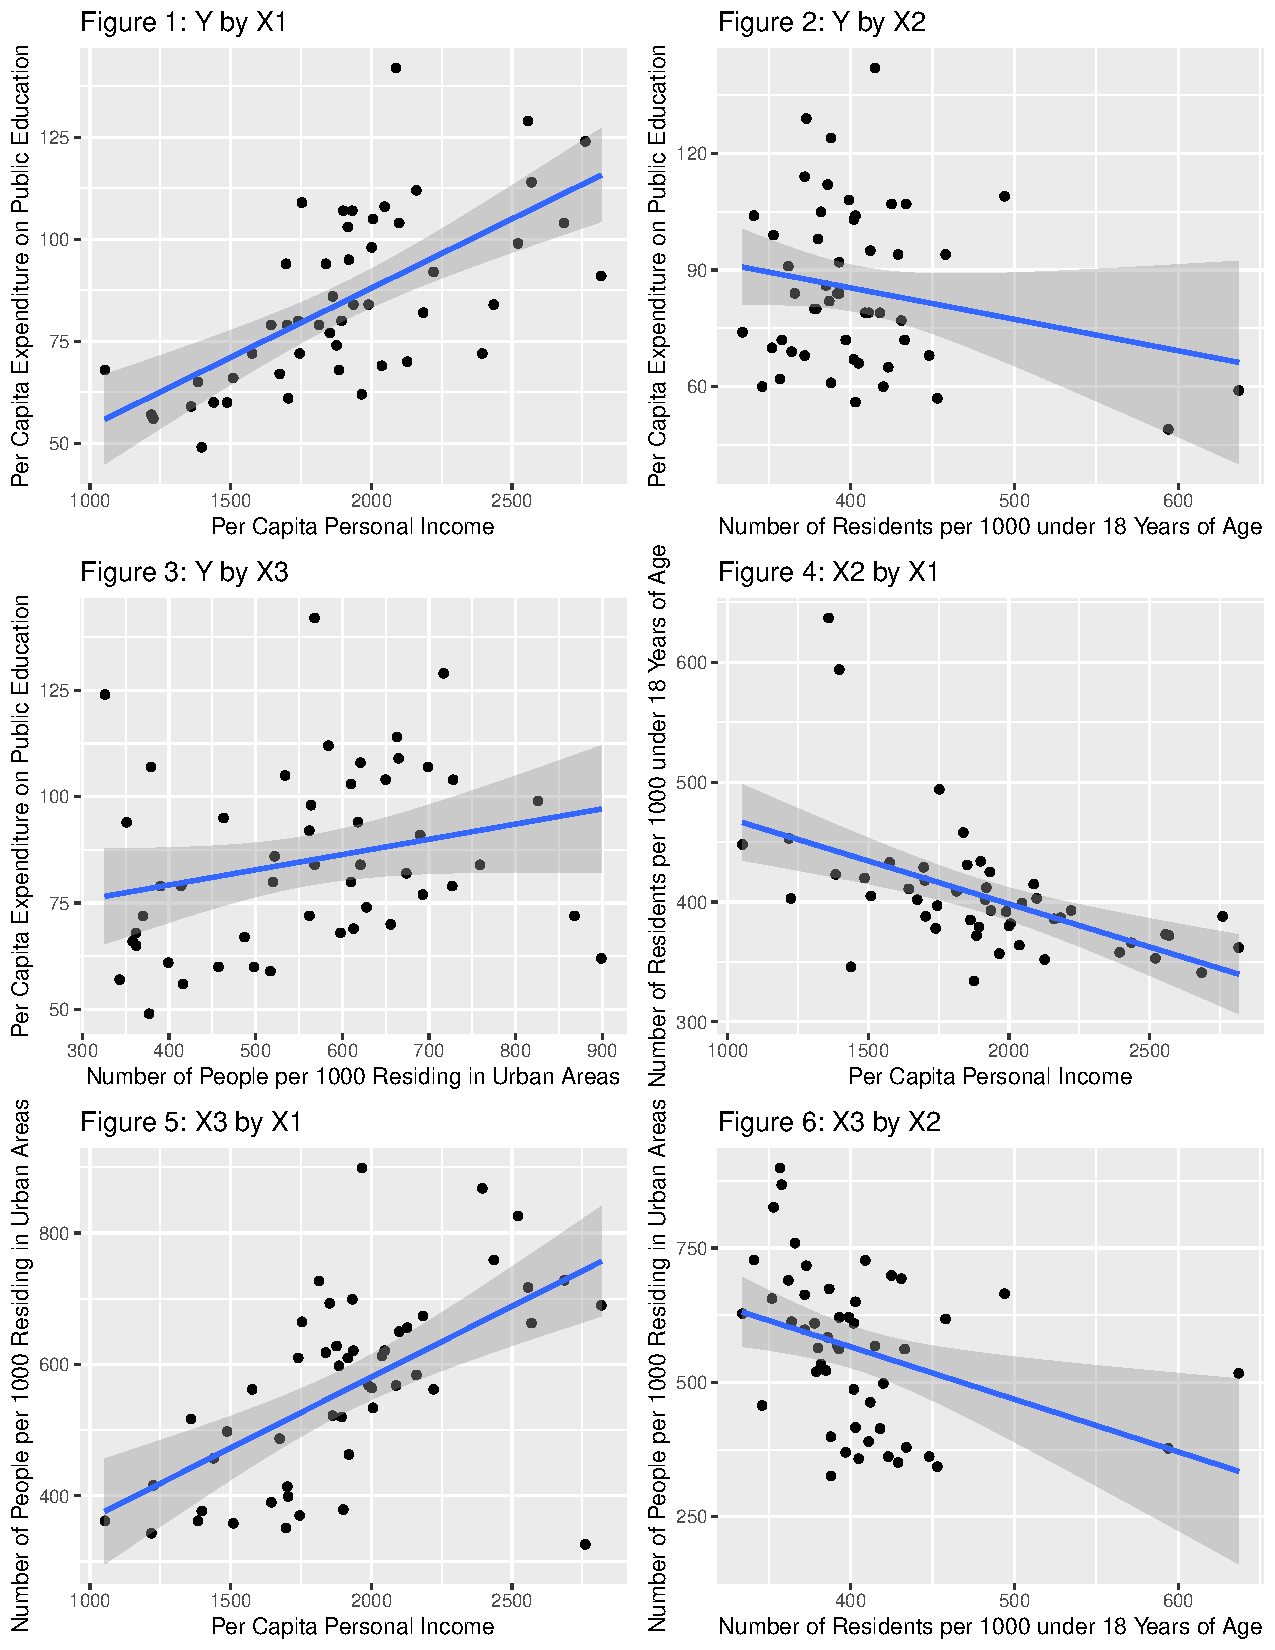
\includepdf[page={1}]{PS1_Graph_1} 

\vspace{.5cm}

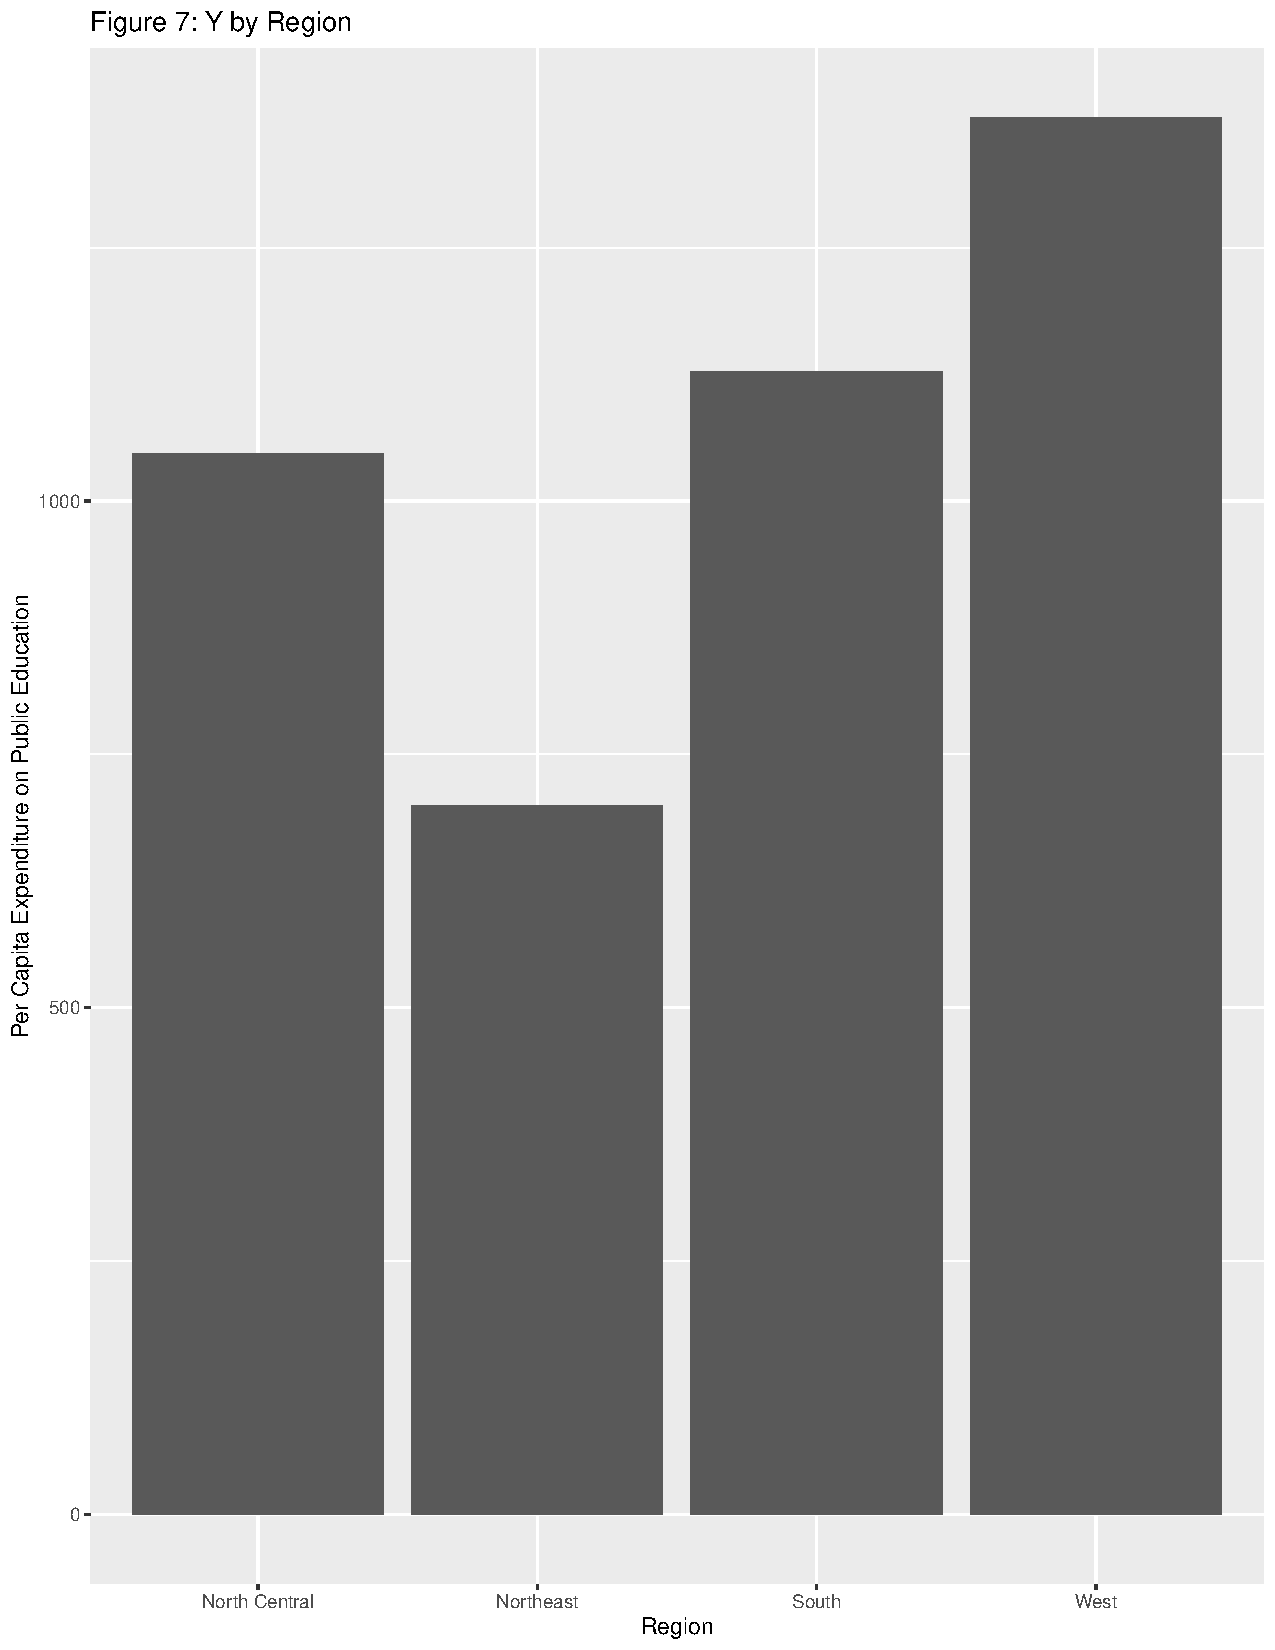
\includepdf[page={1}]{PS1_Graph_2} 

\vspace{.5cm}

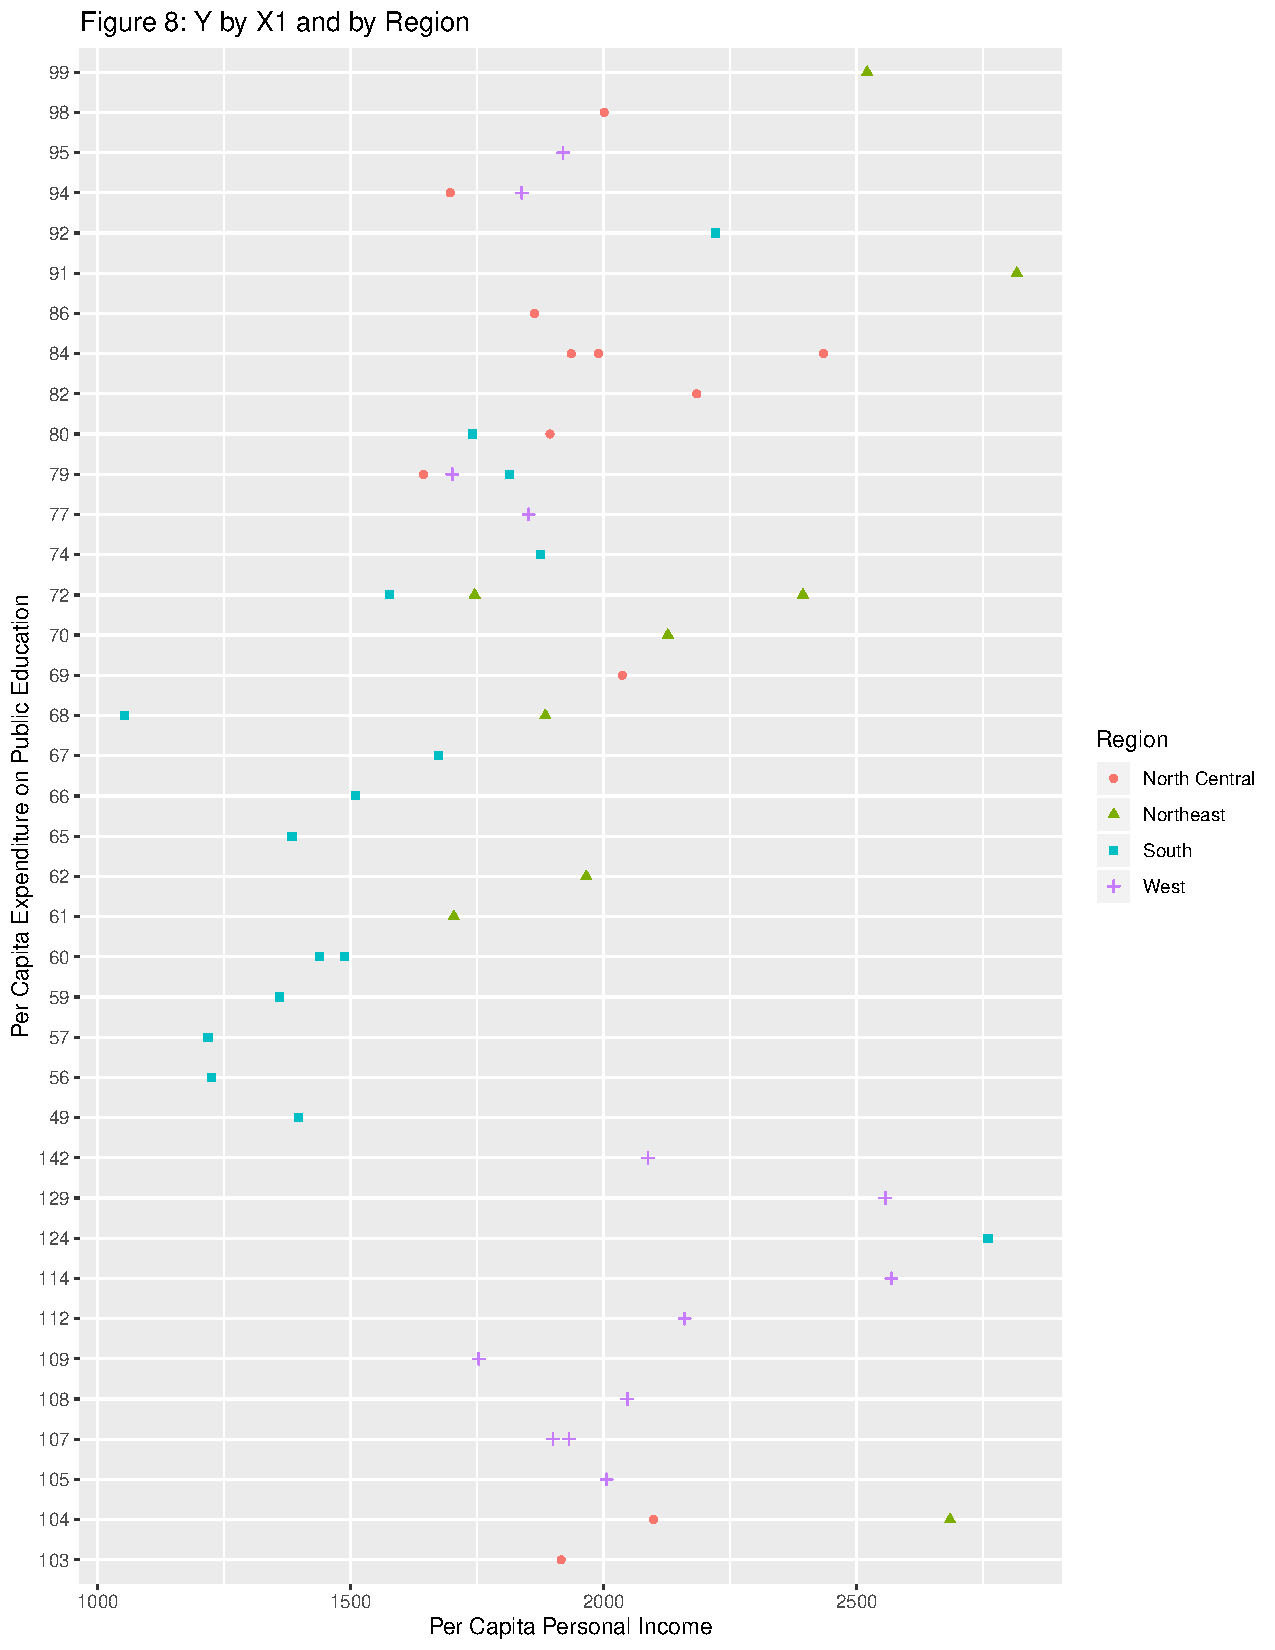
\includepdf[page={1}]{PS1_Graph_3} 

\vspace{.5cm}
\end{document}
